\documentclass{article}
\usepackage{cancel}
\usepackage{amsmath, amssymb, amsfonts}
\usepackage[binary-units]{siunitx}
\usepackage{tikz}
\usepackage{float}
\usepackage{pgffor}
\usepackage{import}
\usepackage{vwcol}
\usepackage{fontawesome}
\usepackage{stmaryrd}
\usepackage{multicol}
\usepackage{pdfpages}
\usepackage{transparent}
\usepackage{xcolor}
\usepackage{scalerel}
\usepackage{stackengine}
\usepackage{algpseudocode}
\newcommand{\diag}{\operatorname{diag}}
\newcommand{\card}{\operatorname{card}}
\newcommand{\tr}{\operatorname{tr}}
\newcommand{\rg}{\operatorname{rg}}
\renewcommand{\epsilon}{\varepsilon}
\newcommand{\equivalent}[1]{\underset{#1}{\sim}}
\newcommand{\R}{\mathbb{R}}
\newcommand{\Q}{\mathbb{Q}}
\newcommand{\C}{\mathbb{C}}
\newcommand{\N}{\mathbb{N}}
\newcommand{\Z}{\mathbb{Z}}
\newcommand{\cM}{\mathcal{M}}
\newcommand{\cO}{\mathcal{O}}
\newcommand{\dx}{\mathrm{d}x}
\newcommand{\dy}{\mathrm{d}y}
\newcommand{\dz}{\mathrm{d}z}
\newcommand{\dt}{\mathrm{d}t}
\newcommand{\df}{\mathrm{d}f}
\newcommand{\Sp}{\operatorname{Sp}}
\newcommand{\dangersign}[1][2ex]{%
  \renewcommand\stacktype{L}%
  \scaleto{\stackon[1.3pt]{\color{red}$\triangle$}{\tiny !}}{#1}%
}

\usepackage[a4paper,top=4cm,bottom=4cm,left=3cm,right=3cm,marginparwidth=1.75cm]{geometry}
% \newcommand{\incfig}[2][1]{%
%     \def\svgwidth{#1\columnwidth}
%     \import{./figures/}{#2.pdf_tex}
% }
% 
\newenvironment{theorem}[1][\unskip]{
	\paragraph{Théorème #1}

}{}

\newenvironment{proof}[1][\unskip]{
	\def\temp{#1}\ifx\temp\empty
		\paragraph{Preuve}
	\else
		\paragraph{Preuve \emph{(#1)}}
	\fi

}{}

\newenvironment{definition}[1][\unskip]{
	\paragraph{Définition: #1}

}{}

\newenvironment{warning}[1][\unskip]
{
	\vspace{1cm}
	\begin{minipage}[c]{0.1\linewidth}
	\dangersign[8ex] 
\end{minipage}%
\begin{minipage}[l]{0.9\linewidth}
}
{
	\end{minipage}
	\vspace{1cm}
}

% \pdfsuppresswarningpagegroup=1


\begin{document}
	\section{Communications numériques}
	\begin{description}
		\item[Chaine de base] 
			\begin{align*}
				\underbrace{\text{bits} \to  \textbf{emetteur} \to \underbrace{\text{signal} \to  \textbf{canal de propagation} \to \text{signal abimé}}_\text{SNR\footnote{signal-to-noise ratio}} \to \textbf{récepteur} \to  \text{bits reçus} }_\text{TEB\footnote{taux d'erreur binaire}}
			\end{align*}
	\end{description}

	\subsection{Avantages \& inconvénients}
	\begin{description}
		\item[Qualité de transmission améliorée] $\text{TEB} = 0$ possible même si $\text{SNR} \neq 0$.
		\item[Nouvelles fonctions] c.f. Codage canal
		\item[Bande passante occupée] la bande de fréquences est bien plus grande, c.f. codage source
	\end{description}
\subsection{Élements de la chaîne de transmission}

\subsubsection{Codage source}

Dans la couche software
On affecte moins de bits aux symboles (e.g. lettres) les plus fréquentes:

Si on a les probabilités suivantes:

\begin{table}[H]
	\centering
	\label{tab:probas-apparition-lettres}
	\begin{tabular}{cc}
	Lettre & Probabilité \\\hline
	A & 0.6 \\
	B & 0.2 \\
	C & 0.1 \\
	D & 0.1
	\end{tabular}
\end{table}

On codera les lettres comme cela:

\begin{align*}
	\begin{cases}
	A &\mapsto 0 \\
	B &\mapsto 10 \\
	C &\mapsto 110 \\
	D &\mapsto 111
	\end{cases}
\end{align*}

\ldots Au lieu d'utiliser un codage naïf $\begin{cases}
	A &\mapsto 00 \\
	B &\mapsto 01 \\
	C &\mapsto 10 \\
	D &\mapsto 11
\end{cases}$

\subsubsection{Codage canal}
Dans la couche physique

On envoie chaque bit en triple pour faire une correction d'erreur par vote au décodage (ou tout autre principe de code correcteur):

\begin{align*}
	0110 \to 000\ 111\ 111\ 000 \to \textbf{canal de propagation} \to 00{\mathbf 1}\ 1\mathbf{00}\ 111\ \mathbf{111} \to 0\mathbf{0}1\mathbf{1}
\end{align*}

Donc 
\begin{description}
	\item[Rendement] 1/3
	\item[Capacité de détection] 2 erreurs
	\item[Capacité de correction] 1 erreur
\end{description}

\subsubsection{Modulation}

Exemple: NRZ modulé

\subsubsection{Synchronisation}

On transmet avec une fréquence porteuse, mais il faut revenir à la fréquence du signal original (on appelle ça le \emph{retour en bande de base}).

Mais les cos/sin qu'on utilise pour revenir sont pas exactement les mêmes  (niveau fréquence et phase) que ceux utiliser pour aller sur la fréquence porteuse.

Il y a aussi des erreurs \emph{sur l'horloge} (en temps): les erreurs de phase sur l'horloge corresponde au fait qu'on commence à transmettre avec un délai, et l'erreur de fréquence sur l'horloge c'est quand la longueur d'un bit (symbole) n'est pas celle attendue par le récepteur.

\subsection{Modulation numérique en bande de base}

\subsubsection{Exemples}

\begin{description}
	\item[Codage élémentaire] On a $T_s = T_b$ (où $T_s$ est la durée d'un symbole, l'élément de donnée transmise et $T_b$ la durée d'un bit, élément de donnée originale)
	\item[Codage bloc] On a $T_s = nT_b, n \in \N^\ast$, par exemple 00 devient +3 V, 01 devient +1 V, 10 devient -1 V et 11 devient -3 V.
	\item[Codage par niveau] Le niveau est constant sur chaque période $T_s$.
	 \item[Codage par transition] Un symbole est transmis comme un changement de niveau, le niveau change exactement une fois au milieu de chaque $T_s$.
\end{description}

\subsubsection{Construction}

\paragraph{Forme d'onde}
Signal élémentaire de durée $T_s$ utilisé pour transmettre. On multiplie ensuite ce signal par quelque chose pour créer les différents symboles.

\begin{figure}[H]
	\centering
	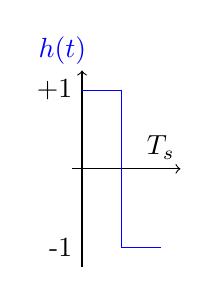
\begin{tikzpicture}[scale=0.125]
		\draw (-2, 12) node[blue]{$h(t)$ };
		\draw[->] (-1, 0) -- (10, 0);
		\draw[->] (0, -10) -- (0, 10);
		\draw[blue] (0, 8) -- (4, 8) -- (4, -8) -- (8, -8);
		\draw (0, 8) node[left]{+1};
		\draw (0, -8) node[left]{-1};
		\draw (8, 0) node[above]{$T_s$};
	\end{tikzpicture}
	\caption{Exemple de la forme d'onde d'Ethernet\footnote{IEEE802.3}}
	\label{fig:}
\end{figure}

\paragraph{Mapping} table de correspondance entre le bit à transmettre et le symbole utilisé.

\begin{table}[H]
	\centering
	\caption{Mapping NRZ\footnote{non-retour à zéro} élémentaire par niveau}
	\label{tab:mapping-élémentaire-niveau}
	\begin{tabular}{cc}
	Bit & Symbole \\\hline
	0 & -1 V \\
	1 & +1 V
	\end{tabular}
\end{table}

On a donc

\begin{align*}
	\text{modulé}(t) &= \sum_{k\in \N} \text{mapping}(\text{bits}_k) \cdot \text{forme d'onde}(t - k T_s)  \\
	&= \sum_{k\in \N} \text{mapping}(\text{bits}_k) \delta(t-kT_s) \ast \text{forme d'onde}(t) \quad&\text{on reconnaît un processus de filtrage!} \\
\end{align*}

$\text{forme d'onde}$ est donc la réponse impulsionnelle d'un filtre appelé \emph{filtre de mise en forme}.

\begin{align*}
	\text{bits} \to  \underbrace{\textbf{mapping} \to \text{symboles} \to \textbf{filtre de mise en forme} }_\text{modulateur bande de base} \to  \text{signal}
\end{align*}

\subsubsection{Débit symbolique/binaire}

Pour coder $n$ bits par symbole, il faut $(\card \{0, 1\})^n = 2^n =: M$ symboles

\paragraph{$M$-PAM (Pulse Amplitude Modulation)}
Ou \emph{modulation par impulsion codée}.

On prend pour symboles $\{\pm \text{V}, \pm 3 \text{ V}, \ldots, \pm (M-1) \text{ V}\} $ 

\begin{align*}
	T_s &= n T_b \\
	\iff \frac{1}{T_s} &= \frac{}{nT_b} \\
	\iff R_s &= \frac{1}{n} R_b \\
	&= \frac{R_b}{\log_2(M)} \\
\end{align*}

\subsection{Densité spectrale de puissance}


La densité spectrale de puissnace vaut

\begin{align*}
	S_x(f) &= \frac{\sigma_a^2}{T_s} |H(f)\^2 + 2 \frac{\sigma_a^2}{T_s} |H(f)|^2 \sum_{k=1}^{\infty} \re(R_a(k) e^{j_2\pi fkT_s}) + \frac{|m_a|^2}{T_s^2} \sum_{k} \left| H\left( \frac{k}{T_s} \right) \right|^2 \delta\left( f - \frac{k}{T_s} \right)   \\
\end{align*}

Où 
\begin{description}
	\item[$\sigma_a^2$] Variance des symboles
	\item[$m_a$] Moyenne des symboles
	\item[$R_a(k)$] Intercorrélation centrée réduite du $k$-ième symbole.
	\item[$H(f)$] Transformée de fourier de la forme d'onde
\end{description}

Dans presque tout les cas en pratique, on a des symboles centrés indépendants, donc $m_a = R_a(k) = 0$ et l'exression ne garde que le premier terme de la somme.

\begin{description}
	\item[Signal ``bande de base"] Signal dont les fréquences sont centrées autour de 0
\end{description}

\subsection{Bande de fréquence occupée par le signal à transmettre $B$}

On a 2 définitions

\begin{itemize}
	\item Bande contenant $x\%$ de l'énergie du signal ($x\in [95, 99]$)
		\begin{align*}
			\frac{\int_0^B  S_x}{\int_0^{\infty} S_x} &= \frac{x}{100} \\
		\end{align*}
	\item Bande au délà de laquelle l'atténuation minimal est de $x\text{ dB}$ ($x\in [20, 30]$)
\end{itemize}

Dans les deux cas
\begin{align*}
	B \propto R_s
\end{align*}

\subsection{Critères de performance}

\begin{description}
	\item[Efficacité en puissance] 
SNR par bit nécéssaire à l'entrée du récepteur pour atteindre un TEB souhaité
\item[Efficacité spectrale $\eta$] Bande nécéssaire pour atteindre un débit binaire souhaité
	\begin{align*}
		\eta &= \frac{R_b}{B}= \frac{\log_2(M)}{k} \\
	\end{align*}
\end{description}

\subsection{Canal de propagation}

Lien physique entre émetteur et récepteur.
On conçoit les émetteurs et récepteurs \emph{en fonction du canal de propagation}. 

\subsubsection{Examples}

\begin{itemize}
	\item Air
	\item Fibre
	\item Câble
\end{itemize}

\subsubsection{Distortions et contraintes}

\paragraph{Atténuation}
Réduction de l'amplitude

\paragraph{Transposition de fréquence}
Pour mettre le signal autour de la porteuse (fréquentiellement)

\paragraph{Multiplexage}
On peut diviser par
\begin{description}
	\item[FDM] fréquences
	\item[CDM] DSP (code spécifique)
	\item[TDM] temps (l'un après l'autre)
	\item[MF-TDM] par fréquences et temps (ou d'autres mélanges)
\end{description}

\paragraph{Plusieurs trajets}

\begin{enumerate}
	\item Chaque trajet a sa propre atténuation $\alpha$, son retard $\tau$ et un bruit $n(t)$

		 \begin{align*}
			y(t) = \alpha x(t-\tau) = \alpha \delta(t-\tau) \ast x(t) + n(t)
		\end{align*}
	\item On reçoit les différents trajets
		\begin{align*}
			y(t) = \sum_{k=0}^{N-1} \alpha_k \delta(t-\tau_k) \ast x(t) + n(t)
		\end{align*}
\end{enumerate}

Le canal de propagation est donc un filtre de réponse impulsionnelle $\sum_{k=0}^{N-1}  \alpha_k \delta(t-\tau_k)$ auquel on a ajouté un bruit (supposé additif blanc\footnote{DSP constante} et Gaussien) $n(t)$.

\subsubsection{Cas d'un canal AWGN\footnote{Additive White Gaussian Noise}}

Cas d'un canal à un seul trajet en vue directe, le filtre est à module constant et déphasage linéaire en fréquence, donc c'est comme s'il n'y avait que du bruit blanc  (d'où le nom)

\subsubsection{Canal AWGN à bande passante limitée}

Le module du filtre est constant sur la bande passante et nul en dehors, le déphasage est linéaire en fréquence sur la bande passante et nul en dehors.

\subsubsection{Canal sélectif en fréquence}

Quand le signal se propage sur plusieurs trajets.

\subsection{Canal non-stationnaire}
Les paramètres changent avec le temps.




\end{document}
